\chapter[Desenvolvimento ]{Desenvolvimento}
Neste projeto foi acordado o Desenvolvimento da tecnologia de Manutenção Remota envolvido no projeto de gestão de embarcados dos ATM’s e TFL’s.
Esta sessão apresenta todas as funcionalidades desenvolvidas ao longo do projeto, logo em seguida, na sessão de
Relatos Diários serão descritos todas as atividades desenpenhadas diáriamente no trabalho.

\section{Verifica\c{c}\~ao de Informa\c{c}\~oes}

\bigskip

{\color{black}
    \ \ \ \ O processo de obten\c{c}\~ao de informa\c{c}\~oes das m\'aquinas da Caixa Econ\^omica Federal sempre foi feita
        de maneira manual, utilizando shell scritps. Foi proposto e implantado o desenvolvimento de um painel de
        monitora\c{c}\~ao e manuten\c{c}\~ao remota dos equipamentos. O primeiro ponto para que a solu\c{c}\~ao fosse
        satisfeita foi executar a manuten\c{c}\~ao remota, resgatando as informa\c{c}\~oes de uma determinada m\'aquina. }

{\color{black}
    \ \ \ \ Primeiramente, o usu\'ario dever\'a indicar qual a ag\^encia que pertence a m\'aquina que \ est\'a sujeita ao
        recolhimento de dados, logo em seguida, escolhendo-a. Est\~ao a a\c{c}\~ao de recupera\c{c}\~ao de informa\c{c}\~oes
        pode ser feita com o seguinte bot\~ao no painel:}

        \begin{center}
        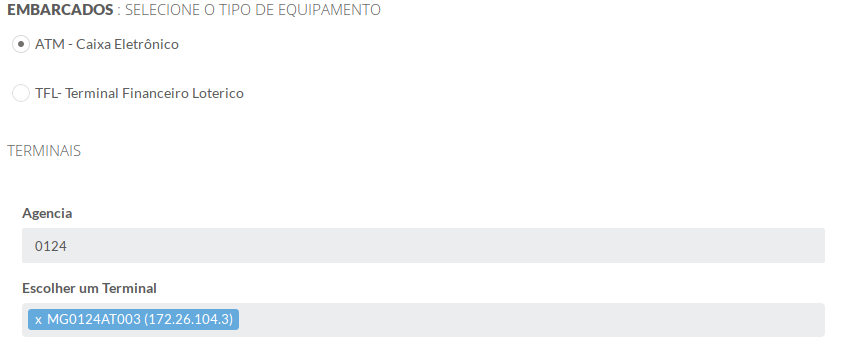
\includegraphics[width=17.029cm,height=7.22cm]{figuras/RATCETECATMSTFLS051718v2-img002.png}
        \end{center}


        \begin{center}
        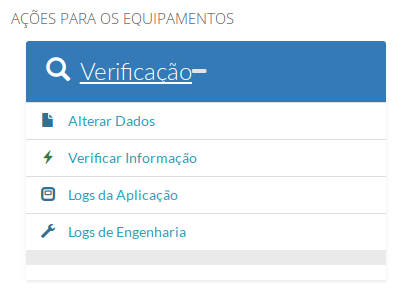
\includegraphics[width=10.82cm,height=7.777cm]{figuras/RATCETECATMSTFLS051718v2-img003.png}
        \end{center}
{\color{black}
    \ \ \ \ Dessa forma, ao solicitar a verifica\c{c}\~ao de informa\c{c}\~oes, o servidor ir\'a recuperar os dados
        atrav\'es do servi\c{c}o ssh na m\'aquina. Ele ir\'a levantar todas as informa\c{c}\~oes e ir\'a apresentar as suas
        informa\c{c}\~oes ao usu\'ario. As informa\c{c}\~oes coletadas ser\~ao as seguintes:}


        \bigskip

{\color{black}
    \ \ }

    \begin{center}
    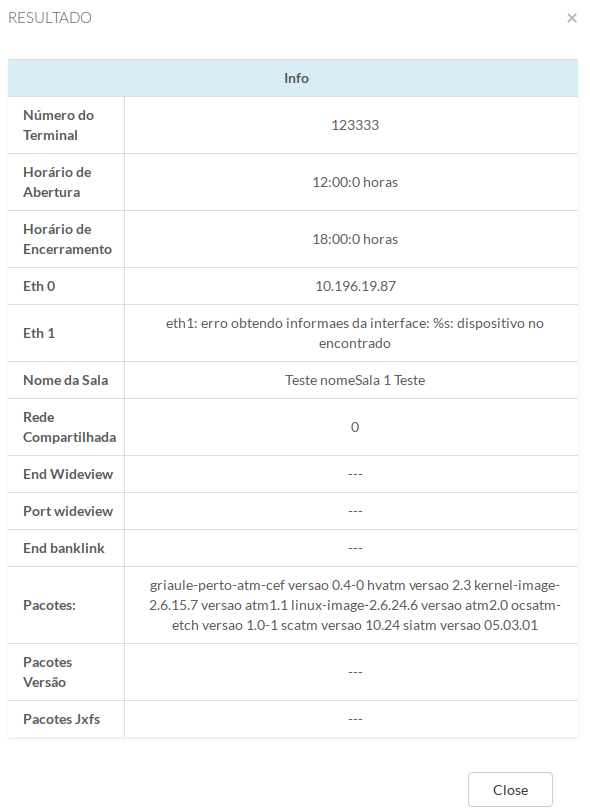
\includegraphics[width=13.936cm,height=19.131cm]{figuras/RATCETECATMSTFLS051718v2-img004.png}
    \end{center}

    \bigskip


    \bigskip

    \section[Altera\c{c}\~ao de Dados]{Altera\c{c}\~ao de Dados}
{\color{black}
    \ \ Para a aplica\c{c}\~ao de altera\c{c}\~ao de dados, no momento, \'e apresentado um formul\'ario que possibilita a
        altera\c{c}\~ao de dados j\'a existentes. Para aplicar uma altera\c{c}\~ao de dados, \'e necess\'ario escolher a
        m\'aquina que receber\'a a mudan\c{c}a.}

{\color{black}
    \ \ Ao escolher o terminal, \'e poss\'ivel selecionar a op\c{c}\~ao para executar a altera\c{c}\~ao, como visto na
        representa\c{c}\~ao a seguir:}

{\color{black}
    \ \ \ \ Sendo selecionada a op\c{c}\~ao, ser\'a apresentado ao usu\'ario o formul\'ario, como dito acima:}

    \begin{center}
    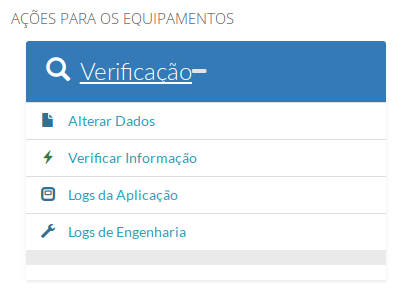
\includegraphics[width=10.82cm,height=7.777cm]{figuras/RATCETECATMSTFLS051718v2-img005.png}
    \end{center}

    \bigskip

{\color{black}
    \ \ Ap\'os o preenchimento do formul\'ario com as devidas informa\c{c}\~oes, estas ser\~ao enviadas para o servidor e
        aplicadas na respectiva m\'aquina. Assim, ir\'a ser criada uma barra de carregamento na parte inferior do site que
        apontar\'a o status atual da tarefa, sendo em progresso ou conclu\'ido. }

        \begin{center}
        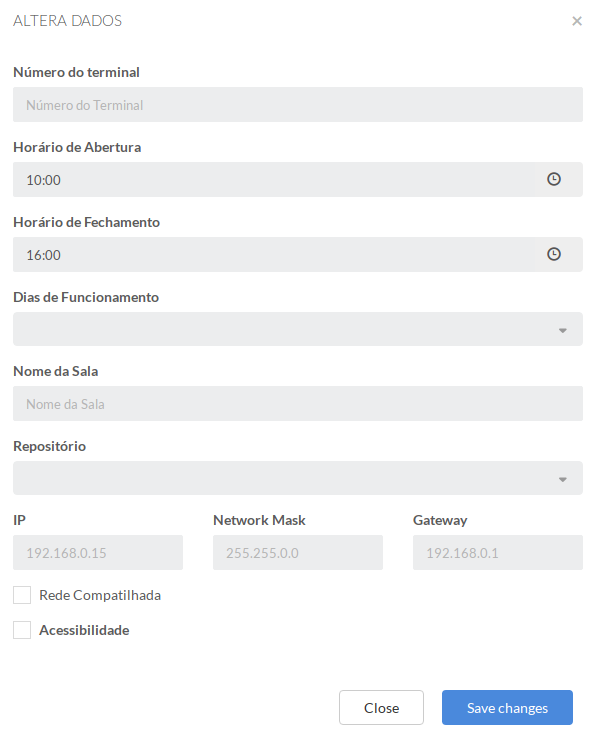
\includegraphics[width=15.279cm,height=18.83cm]{figuras/RATCETECATMSTFLS051718v2-img006.png}
        \end{center}

        \bigskip


        \bigskip


        \bigskip

{\color{black}
    \ \ Ao ter a tarefa finalizada, ser\'a apresentado o status de conclu\'ido e de visualiza\c{c}\~ao dos logs.}

    \begin{center}
    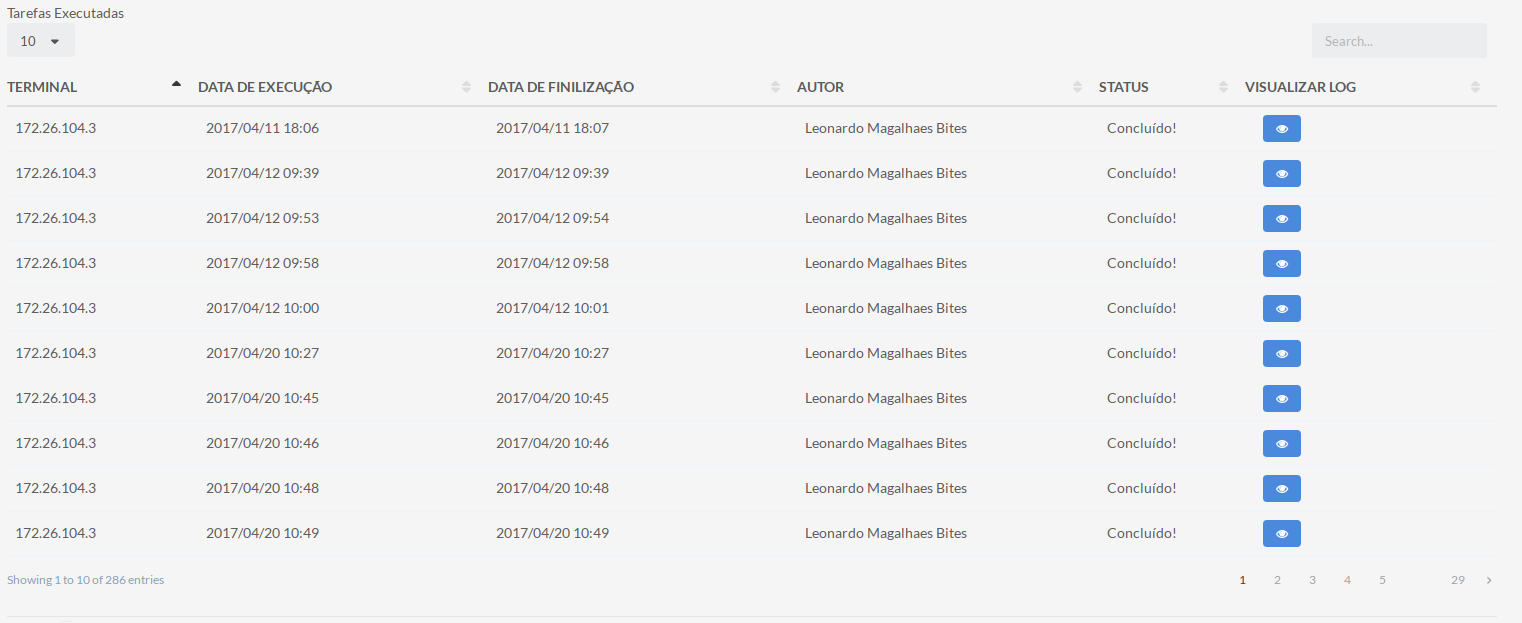
\includegraphics[width=17.029cm,height=6.969cm]{figuras/RATCETECATMSTFLS051718v2-img007.png}
    \end{center}

    \bigskip

    \section{Salvar Logs}
{\color{black}
    \ \ A funcionalidade de salvar log tem como objetivo principal recuperar dois tipos de logs dos terminais. O primeiro
        deles s\~ao os logs da aplica\c{c}\~ao SIMMA, sendo que o segundo s\~ao os logs de engenharia. }

{\color{black}
    \ \ Ap\'os escolher o terminal, que ter\'a o log recolhido, existem duas op\c{c}\~oes para a recupera\c{c}\~ao dos logs,
        como dito a pouco. Estas est\~ao dispostas como exemplificado na tela a seguir:}


        \bigskip

{\color{black}
    \ \ Ao solicitar uma das duas aplica\c{c}\~oes de logs, ser\'a enviada uma solicita\c{c}\~ao para as m\'aquinas, que
        ir\~ao armazenar os dados e enviar para o site. Assim, ser\'a indicado na barra de status, mencionada a pouco, que foi
        finalizada a tarefa com sinal de conclu\'ida. O usu\'ario dever\'a selecionar a op\c{c}\~ao de visualizar log e, logo
        em seguir, baixar o log. }

        \begin{center}
        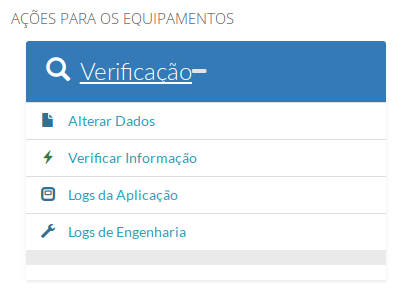
\includegraphics[width=10.82cm,height=7.777cm]{figuras/RATCETECATMSTFLS051718v2-img008.png}
        \end{center}

        \bigskip

        \section{Manuten\c{c}\~ao}
{\color{black}
    \ \ A manuten\c{c}\~ao permite que os terminais tenham manuten\c{c}\~oes pr\'e definidas. Estas podem ser aplicadas em
        v\'arios terminais ao mesmo tempo. \ Estes terminais devem ser escolhidos e assim, podem ser abordadas as
        manuten\c{c}\~oes, que est\~ao dispon\'iveis de acordo com a imagem do servidor a seguir:}


        \bigskip

        \section[Aspectos T\'ecnicos]{Aspectos T\'ecnicos}
        \begin{center}
        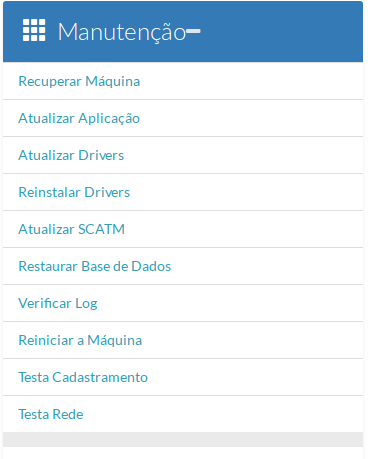
\includegraphics[width=9.793cm,height=12.143cm]{figuras/RATCETECATMSTFLS051718v2-img009.png}
        \end{center}
{\color{black}
    \ \ A seguir ser\~ao apresentados os procedimentos sistem\'aticos, que foram implementados para possibilitar o
        cumprimento dos requisitos desejados pelo cliente. Os cap\'itulos a seguir ser\~ao divididos bem como a arquitetura do
        software. O primeiro cap\'itulo ir\'a apresentar a parte de apresenta\c{c}\~ao, bem como HTML, CSS e JS. O segundo
        cap\'itulo apresentar\'a as views, que fazem e exercem o controle dos procedimentos solicitados ao servidor. Por fim,
        ser\~ao apresentados os procedimentos de implementa\c{c}\~ao nas modelos e scripts de execu\c{c}\~ao. }


        \section[Camada de Apresenta\c{c}\~ao]{Camada de Apresenta\c{c}\~ao}
{\color{black}
    A seguir ser\~ao apresentados os c\'odigos procedurais de apresenta\c{c}\~ao do site. O primeiro apresentado ser\'a a
        tela de index.html da tela de manuten\c{c}\~ao.} Os códigos estão no Anexo \ref{ane:um}.

        

    \section{Camada de Controle dos Dados}
{\color{black}
    Nos scripts a seguir, ser\~ao apresentados todos os procedimentos do servidor que manipulam o controle e direcionamento
        dos dados.}

{\color{black}
    O primeiro a ser apresentado ser\'a o arquivivo de views.py:}
Os códigos estão no Anexo \ref{ane:dois}.

    \section{Camada de Execu\c{c}\~ao}
{\color{black}
    Ser\~ao apresentados todos os scripts para a implementa\c{c}\~ao de aplica\c{c}\~ao de altera\c{c}\~oes de dados nas
        m\'aquinas.}

{\color{black}
    O primeiro apresentado, ser\'a a modelo de heran\c{c}a, como base para todos os outros comandos.}
Os códigos estão no Anexo \ref{ane:tres}.

    \section{Execu\c{c}\~ao dos Servi\c{c}os}
{\color{black}
    Para iniciar a aplica\c{c}\~ao, \'e necess\'ario apenas executar o comando de start da aplica\c{c}\~ao:}

{\ttfamily\color[rgb]{0.10980392,0.10980392,0.10980392}
    python run.py}

\section{Relato Diário}
\label{sec:relato_di_rio}

Nesta sessão serão detalhadas as atividades desenvolvidas para entregar o
projeto dos ATM's e TFL's.

\begin{itemize}
    \item O celery está integrado e configurado na aplicação. Foi elaborado um Vagrantfile
 utilizando receita chef para a automatização da VM. Elaborei um script client padrão para verificar o status
 do celery continuamente. Amanhã irei estabelecer os links entre as tasks com os scripts escritos pelo
 @Leonardo Bites.

    \item A integração foi feita com as tarefas de montagem da imagem. Estão funcionando
  paralelamente à solicitação do usuário. O status da tarefa está sendo apresentado no cliente utilizando
  ajax. Os próximos passos giram em torno do armazenamento dos dados das imagens no banco e a
  aplicação do mesmo procedimento do celery para as tarefas que executam comandos.


    \item As imagens geradas estão tendo suas informações salvas no banco de dados e
  recuperadas ao carregar a página. Foi gerada uma pasta de logs, onde estes arquivos são armazenados de
  acordo com o respectivo ID da imagem no banco. Foi criada uma modal usando jquery e ajax para
  apresentar o log da respectiva imagem. 
  Amanhã irei capturar o arquivo de log e apresentá-lo na respectiva modal.


    \item Toda a etapa de geração de imagens foi finalizada, bem como a apresentação dos logs via ajax. Foi criado o script de migração do banco para inserir uma tupla de configuração do Ldap no momento da criação das tabelas.
  Assim, eu e o @Leonardo Bites, iremos iniciar a parte da manutenção remota.


    \item 18/01 - @Rodrigo Tornis
  Quanto a requisitos funcionais, apliquei uma regra de negócio para só criar uma tupla de configuração no banco de dados se este estiver sem nenhum dado. Quanto a requisitos não funcionais, foi aplicada uma melhoria no layout da página de geração de imagens e no menu. Quanto a requisitos técnicos, foi aplicada a folha de estilo do python, PEP8, em todo o código e foi elaborada a documentação dos métodos ligados à geração de imagem.


    \item 19/01 - @Rodrigo Tornis @Gabriela Dias
  A conexão do python com o celery foi melhorada utilizando Flask Application Factory Pattern. Foi criado um novo módulo para o gerenciamento da manutenção das máquinas. Adicionados as rotas, as views e templates com o respectivo formulário. Foram elaborados scripts js, utilizando ajax, para o envio das tasks de forma assíncrona. No dia 20 será executada a integração das chamadas ajax de manutenção com o celery.


    \item 20-01 @Rodrigo Tornis @Gabriela Dias
  No novo módulo de manutenção, foram adicionadas rotas para acessar os métodos de rederização de página e de acesso do celery. Foram adicionados os forms de manutencao, templates e scripts js. As tasks do celery foram criadas e utilizadas para executar as atividades de manutenção. Foi criada uma classe de histórico de manutenção, para armazenar em persistência quais os comandos foram executados. Foram adicionadas as novas tabelas, via ajax, para as novas chamadas de manutenção.
  No dia 23/01 serão criados os links entre os comandos do dashboard e os comandos para execução do fabric. A interface e a usabilidade com a tabela será trabalhada.


    \item 23/01
  Foi executada a melhoria de aplicar as rows da tabela de imagens dentro da instancia atual da DataTable. Os históricos armazenados foram recuperados da persistência e apresentados no template.


    \item 24/01 - Foram feitos ajustes nas tabelas datatable para melhorar a usabilidade e para adicionar novas rows à table utilizando a classe DataTable.


    \item 25/01 - Foram feitas novas chamadas de log para a página de manutenção. A forma de armazenamento dos logs foi alterada para se adequar mais ao contexto da manutenção. Foi acrescentado na tabela do banco, views e templates a nova coluna de usuário. Os templates sofreram uma retiradas de dados desnecessários. O formado de impressão das datas foi alterado. Foi criada uma nova engine do banco de dados OCS-DW, para coletar as informações das máquinas que serão tratadas pelo sistema.


    \item 26/01 - Ao carregar executar a query select da engine do OCS-DW, foi constatado a inviabilidade do seu uso direto. A query se fez grande o suficiente para deixar o sistema lento. Assim, solicitei auxilio de @Leonardo Bites para encontrarmos uma solução melhor. Ficou decidido que trocaríamos de banco e faríamos algumas consultas ajax das maquinas do OCS. O banco foi trocado e o script js para as consultas foi iniciado.


    \item 27/01 - O código do cliente foi refatorado, retrabalhando as referências erradas. Foram adicionadas bibliotecas, removidas algumas e outras tiveram apenas mudanças de versão. A versão do JQuery estava antiga, na versão 1.11. Não foi possível migrar para a versão 3.1 pois algumas libs, fortemente acopladas ao JQuery não funcionavam bem. Porém, a verão 2.2.4 foi compatível com alguns ajustes.


    \item 13/02 -
  Iniciei os estudos da lib js select2 para fazer buscas dinâmicas pelas máquinas na página da manutenção. Consegui apresentar as buscas utilizando dados pré-selecionados. Agora, estou na transição entre dados estáticos e uso de Ajax.


    \item 14/02 -
  Me deparei com uma dificuldade no momento de utilizar a lib select2 com dados dinâmicos. Ela opera perfeitamente com dados estáticos, porém, quando utilizo Ajax, a mesma não se comporta bem. O problema que estou tendo é incomum, encontrei apenas dois tópicos falando sobre este, todos, sem solução. Para tentar solucionar, criei um post no StackOverflow, lá tem mais informações sobre a problemática. http://stackoverflow.com/questions/42227138/ajax-select2-dont-send-request

  Enquanto isso, iniciei estudos para a otimizar a query de leitura dos ips de todas as máquinas no banco do OCSDW. Agora estou no passo de criar uma tabela intermediária,apenas com os dados que necessitamos e não replicados, no db da aplicação que estamos desenvolvendo. Estou estudando sobre FEDERATED Storage Engine, do MySQL, para executar este passo.


    \item 15/02 -
  Os estudos do FEDERATED foram concluídos e começamos a implementar a rotina para interligar os dois bancos.
  Enquanto isso, surgiu a necessidade de elaborar o dashboard do gerenciamento de tokens com as comunicações via Ajax. Eu e o @Leonardo Bites terminamos de elaborar os métodos da modelo de Tokens e elaboramos as views, ligadas ao template de apresentação. Já é possível visualizar todos os tokens e gerá-los via Ajax.


    \item 16/02 -
  Obrigado, @Gabriela Dias.
  A geração de tokens foi ajustada para mostrar em conjunto tanto os tokens já gerados anteriormente quanto aqueles lançados pelo JQuery.
  Foi implementada a funcionalidade para remover qualquer token via Ajax.
  Foi implementada a funcionalidade de gerar um pdf do token selecionado, este é gerado unicamente no cliente, e não é armazenado no sistema, pois é construído com os atributos de um token.


    \item 17/02 -
  Foi verificado que o botão de impressão do token não estava funcionando corretamente nos tokens gerados via ajax, apenas nos que eram renderizados pela página, este erro foi corrigido.
  Foi iniciado o processo para listar as máquinas que podem ter o token gerado a partir de uma agência informada pelo usuário. Como as otimização para o select ainda não estão prontas, a consulta no banco está demorando aproximadamente 11 segundos. Enquanto a otimização não é finalizada, está sendo implementado um loader para que o usuário aguarde até que a pesquisa seja feita.


    \item 20/02 -
  O framework que estamos utilizando para os templates possui um loader padrão, o qual estava tentando configurar para a funcionalidade. Porém, esse loader é engessado para funcionar apenas quando a página é carregada e isso não nos servia. Assim, foi necessária a implementação por completa de um loader, com as animações, cores(css) e tempos de resposta.
  Enquanto isso, fizemos mais melhorias na query para resgatar as máquinas de uma dada agência, porém, continua lenta. O @Leonardo Bites desconfia sobre a integridade do banco. Iremos mais investigar amanhã.


    \item 21/02 -
  Finalmente foi encontrada a real causa da lentidão das querys. Verificamos que existe uma grande inconsistência no banco do OCS. Os dados estão repetidos por inúmeras vezes. São cerca de 30 mil máquinas que serão monitoradas para a geração de token, porém, a base do ocs conta com 5 milhões de tuplas armazenadas. Para otimizar a query, resolvemos criar outra tabela apenas com os dados únicos das máquinas. O número de rows caiu para cerca de 30 mil. Assim, a nova pesquisa está levando 0.04 segundos para ser executada.
  Quanto a criação dos tokens, hoje foi implementada a funcionalidade para enviar SMS's para os técnicos contendo o nome das máquinas e seu respectivo token. Está funcionando de forma assíncrona, solicitando ao usuário que insira o número de telefone para qual o sms deve ser enviado.


    \item 22/02 -
  Com o término das atividades do token, foram iniciadas as atividades de desenvolvimento de imagens e manutenção. Foi criado um módulo de Html separado para resgatar as máquinas da base do ocs e agora utilizado em várias partes do código.
  Com a atualização da tabela de imagens para DataTable, foi necessário executar uma refatoração do código no momento do update dos dados vindos do status do celery.


    \item 23/01 -
  Começamos a desenvolver a funcionalidade para adicionar pacotes à imagem a critério do usuário. O problema para usar o file uploader do template persistiu e foi decidido iniciar a implementação do nosso próprio módulo para executar uploads dos arquivos. Os arquivos estão sendo selecionados no browser e armazenados no sistema. O próximo passo será elaborar uma forma de ligar os arquivos as imagens.
  O @Leonardo Bites executou as rotinas diretamente no banco para todos os dias atualizar a tabela. vamos verificar amanhã se tudo ocorreu corretamente.


    \item 24/02 -
  Hoje verificamos a base de dados para verificar se a rotina foi executada com sucesso. Foi verificado que não, a causa foi identificada e mitigada. Executamos novamente e no próximo dia útil será verificado se esta funcionou corretamente.
  Quanto a questão do upload dos arquivos, foram feitas validações para permissão de arquivos apenas de extensão .deb. Foi implementada a funcionalidade para apresentar o progresso do upload. Foi adicionada a funcionalidade para arrastar arquivos diretamente.


    \item 01/03 -
  Foi executada uma extensa refatoração no código com o intuito de aumentar a sua manutenibilidade. Foram refatorados, de acordo com a pep8, todos os arquivos python do projeto; todos os arquivos de script js relativos à manutenção, token e imagens; todos os arquivos html relativos à manutenção, token e imagens.


    \item 02/03 -
  Foi implementada uma rotina para criação de de pastas temporárias que venham a armazenar os respectivos pacotes que irão integrar cada imagem. Estas pastas estão sendo criadas no servidor da aplicação e excluídas quando recebem a respostar que o processo executado pelo fabric foi finalizado.
  No escopo das manutenções remotas, os scripts para apresentação de notificações foram modularizados em um arquivo a parte e modificados para que suportassem polimorfismo.
  Foi implementada uma regra de negócio que, além de não permitir que seja executada uma manutenção caso não sido escolhidos um terminal, é apresentada ao usuário uma notificação de erro.


    \item 06/03 -
  Discutindo sobre a aplicação, verificamos a necessidade de adicionar uma regra de negócio à fila das imagens. Os tipos de imagens(ATM, SIPNL, TFL) podem ser gerados simultaneamente, porém, duas imagens do mesmo tipo não podem ser geradas concomitante. Assim, foram analisadas as configurações do celery. Foi implementada uma alternativa para o problema, que é levantar 3 instâncias de worker do celery, uma para cada máquina e permitindo que cada worker tenha apenas uma tarefa simultânea. Apesar de ser viável, a equipe não acredita que é uma boa solução e será analisado na segunda a viabilidade de executar outro caminho.


    \item 08/03 -
  Foi investigado mais investigado sobre como ter várias queues com número de concorrência distintos. Encontrei uma issue no git hub de muitas pessoas pedindo para ser implementada a feature no celery, pois ela ainda não existe. Abaixo, o desenvolvedor ressaltou sobre a melhor forma, até o momento, de resolver o problema. Felizmente a melhor maneira foi a que adotamos, assim, não foram houve alteração de código. A justificativa pode ser vista com mais detalhes aqui: https://github.com/celery/celery/issues/1599

    \item A aplicação foi colocada em produção, foram encontrados alguns problemas no wsgi, mas resolvemos.

    \item Foi criada uma interface json para validar um token com uma máquina. A interface é um método get que recebe dois parâmetros, máquina e token, e o valida, retornando true ou false com um json.

    \item Foram adicionados aos logs das imagens os nomes de todos os pacotes que foram geradas com ela.


    \item 09/03 -
  Foi verificado que existe a possibilidade que uma máquina ainda não tenha seu nome, porém, precisará de um token para efetuar a instalação. Assim, o front-end foi redesenhado no momento da criação do token para que disponibilizasse ao usuário a opção de cadastrar uma nova máquina. O novo código da máquina já está integrado ao procedimento de geração de tokens.

  Amanhã será executada a rotina de verificação e criação desta máquina em persistência.


    \item 10/03 -
  A rotina de verificação e criação das máquinas foi executada com sucesso, finalizando essa feature.
  Todos os tokens gerados e não utilizados ficam em persistência, porém, o usuário só tem acesso aos válidos do dia.
  Foram formatados campos de datas e reordenados para a geração de imagens.
  Foi iniciada a migração dos scripts para código python, utilizando fabric. Foi criada uma classe para lidar com todos os comandos, esta classe pai foi finalizada. Agora está sendo trabalhada uma de suas especializações, InformationCommand, que recupera algumas informações da máquina(ATM, TFL).


    \item 13/03 -
  Foi continuada a implementação da classe InformationCommand, todos os comandos foram escritos em python. Foi criada uma nova classe Information para armazenar e organizar todas as informações obtidas. Esta foi desacoplada de InformationCommand, pois os comandos não são do mesmo domínio das informações, por isso, duas classes.
  Foi observado que as classes estavam extensas, assim, poderia ser que carecessem de refatoração. Para basear a refatoração, foram utilizados indicadores para análise estática de código, indicando a: complexidade ciclomática(CC); Maintainability Index; LOC; LLOC; SLOC.
  Para CC, o código teve nota máxima.
  manutencao/information.py
  LOC: 191
  LLOC: 108
  SLOC: 209
  Comments: 6
  Single comments: 8
  Multi: 9
  Blank: 44

  Comment Stats
  (C \% L): 3\%
  (C \% S): 3\%
  (C + M \% L): 8\%
  Para Maintainability Index: manutencao/information.py - A (58.23)
  Certificando a qualidade do código, mesmo sendo extenso. Assim, pelos índices de qualidade das métricas recolhidas, a refatoração não foi executada.


    \item 14/03 -
Foi iniciada a implementação da classe para alteração dos dados, ChangeDataCommand. Foram observados que alguns métodos utilizados em InformationCommand também seriam reutilizados. Dessa maneira, estes métodos foram escritos na classe generalista(Command). A primeira opção para a alteração de dados, ChangeTerminalNumber, teve a implementação iniciada. Amanhã a implementação desta classe será retomada e será testada a classe InformationCommand diretamente no ATM.


    \item 15/03 - @Gabriela Dias, quanto a pergunta 1, estou transcrevendo os scripts de manutenção para fabric, bem pythonico.


    \item 21/03 -
Todos os scripts de informações e alteração de dados foram implementados e testados.
Agora os scripts de manutenção estão sendo implementados. Amanhã serão finalizados e testados.


    \item 22/03 -
Os scripts de manutenção foram finalizados. Houve indisponibilidade do ATM de testes, assim, não foi possível testá-lo. Enquanto isso, os scripts para salvar log começaram a ser implementados.


    \item 23/03 -
A implementação dos scripts de Salvar log foi continuada. Os scripts de manutenção foram testados e verificou-se a necessidade de aplicar um repositório para o ATM. Sem o repositório não tem como baixar e atualizar pacotes.


    \item 24/03 -
Foram implementados os scripts de recolha de log para máquinas da fabricante Perto.


    \item 27/03 -
Foram implementados os scripts de recolha de log para máquinas da fabricante Procomp.


    \item 28/03 -
Os scripts de log foram finalizados. Foram iniciados os testes no ATM e melhorias corretivas foram aplicadas. Amanhã os testes irão prosseguir.


    \item 29/03 -
Os scripts menores foram testados e estão funcionando perfeitamente. A geração de logs da perto foi testada, ajustada e está funcional.


    \item 31/03 -
Os scripts foram todos testados e concluídos.


    \item 04/04 -
Foram definidas datas para as próximas atividades.
Salvar logs \& Atualização de repositório (18/04)
Resgatar informações \& Alteração de dados (05/05)


    \item 05/04 -
Foi desenhada e criada a categoria de fila do celery para executar as tarefas paralelamente. Está sendo implementado o método de despache da execução dos comandos.


    \item 06/04 -
Foi implementado um script manage, para criar arquivos de migração e aplicá-las no banco, melhorando o processo de alteração do DB.
Foi implementada a solicitação e a escrita do log do script para salvar logs de engenharia.
Foi adicionado o padrão do link do resultado do método na model.


    \item 10/04 -
Foi estabelecido corretamente o sistema de disponibilização de arquivos globalmente, para todos os entry points que solicitam uma tarefa remota.


    \item 11/04 -
Foi implementada a funcionalidade de apresentação do log salvo via método manage-log, que apresenta todos os logs, seja os que estão carregados dinamicamente na página ou os que foram recuperados do banco de dados.


    \item 12/04 -
Foram finalizadas todas as funcionalidades de logs.


    \item 13/04 -
Foi iniciada a implementação das funcionalidades de gerenciamento de repositório. Os devidos links formam criados e estão sendo mapeados nos scripts.


    \item 18/04 -
Foi finalizada a parte de frontend dos repositórios.


    \item 19/04 -
Foi iniciado o frontend para a verificação de informações. Foi encontrado um missmatch na resposta do servidor no momento do retorno das tasks do celery para esta parte. Foi iniciado um novo processo de definição e implementação desta funcionalidade.


    \item 20/04 -
Foi finalizada a arquitetura para receber o backend para a verificação das informações. A model Information foi ajustada para ser serializada e já está sendo enviada ao cliente.


    \item 24/04 -
A apresentação de informações foi recebida no frontend e está sendo elaborado o jquery para apresentação destas.


    \item 25/01 -
A apresentação de informações das máquinas foi finalizada.


    \item 26/04 -
Foi iniciada a elaboração do frontend para a alteração das informações. Os formulários estão sendo elaborados.


    \item 02/05 -
O html/css/js está totalmente pronto. Agora estão sendo transmitidos os dados dos templates para as views, dentro do celery.


    \item 04/05 -
Os dados estão sendo migrados para o backend. Ocorreram algumas inconsistências no parser dos dados do número do terminal e seus horários. Estes problemas foram resolvidos. Amanhã serão aplicados os dados para acessibilidade e rede compartilhada.


Todas as funcionalidades esperadas do Altera Dados estão implementadas. Estão sendo aplicados pequenos ajustes finos na apresentação dos dados.


Foi concluída a implementação para iniciar os workers do celery quando se inicia a aplicação.


    \item 15/05 -
        O RAT da etapa 1.8 foi finalizado e encontra-se disponível nos files das Tasks.
Algumas considerações foram feitas por parte do cliente:

\begin{enumerate}
    \item Executar validação se a imagem contém os pacotes mínimos.
    \item Incluir nos logs do usuário os protagonistas das ações.
    \item Cancelar geração de imagem
    \item Gerar tokens para todos os terminais de uma agência
    \item Valores do Alterar dados com preenchimento
    \item Trocar valores de acessibilidade para sim ou não
    \item Remover ip do alterar dados
    \item Aplicar ações no log de manutenção
    \item Executar 'dpkg -a' antes de executar qualquer manutenção
\end{enumerate}
\end{itemize}
